%%%%%%%%%%%%%%%%%%%%%%%%%%%%%%%%%%%%%%%%%%%%%%%%%%%%%%%%%%%%%%%%%%%%%%%%%%%
\chapter{Results and Discussion}
%%%%%%%%%%%%%%%%%%%%%%%%%%%%%%%%%%%%%%%%%%%%%%%%%%%%%%%%%%%%%%%%%%%%%%%%%%%

This chapter presents the training results and performance evaluation of the MARQ framework across different phases of the curriculum. The evaluation focus is on the agent's ability to acquire tactical knowledge and manage imperfect information.

\section{Training Progress and Convergence}

Training was conducted over 34,000 episodes, following the five-phase curriculum. Figure \ref{fig:training_progress} illustrates the convergence behavior of the Rainbow DQN agent.

\begin{figure}[htbp]
    \centering
    \begin{subfigure}[b]{0.48\textwidth}
        \centering
        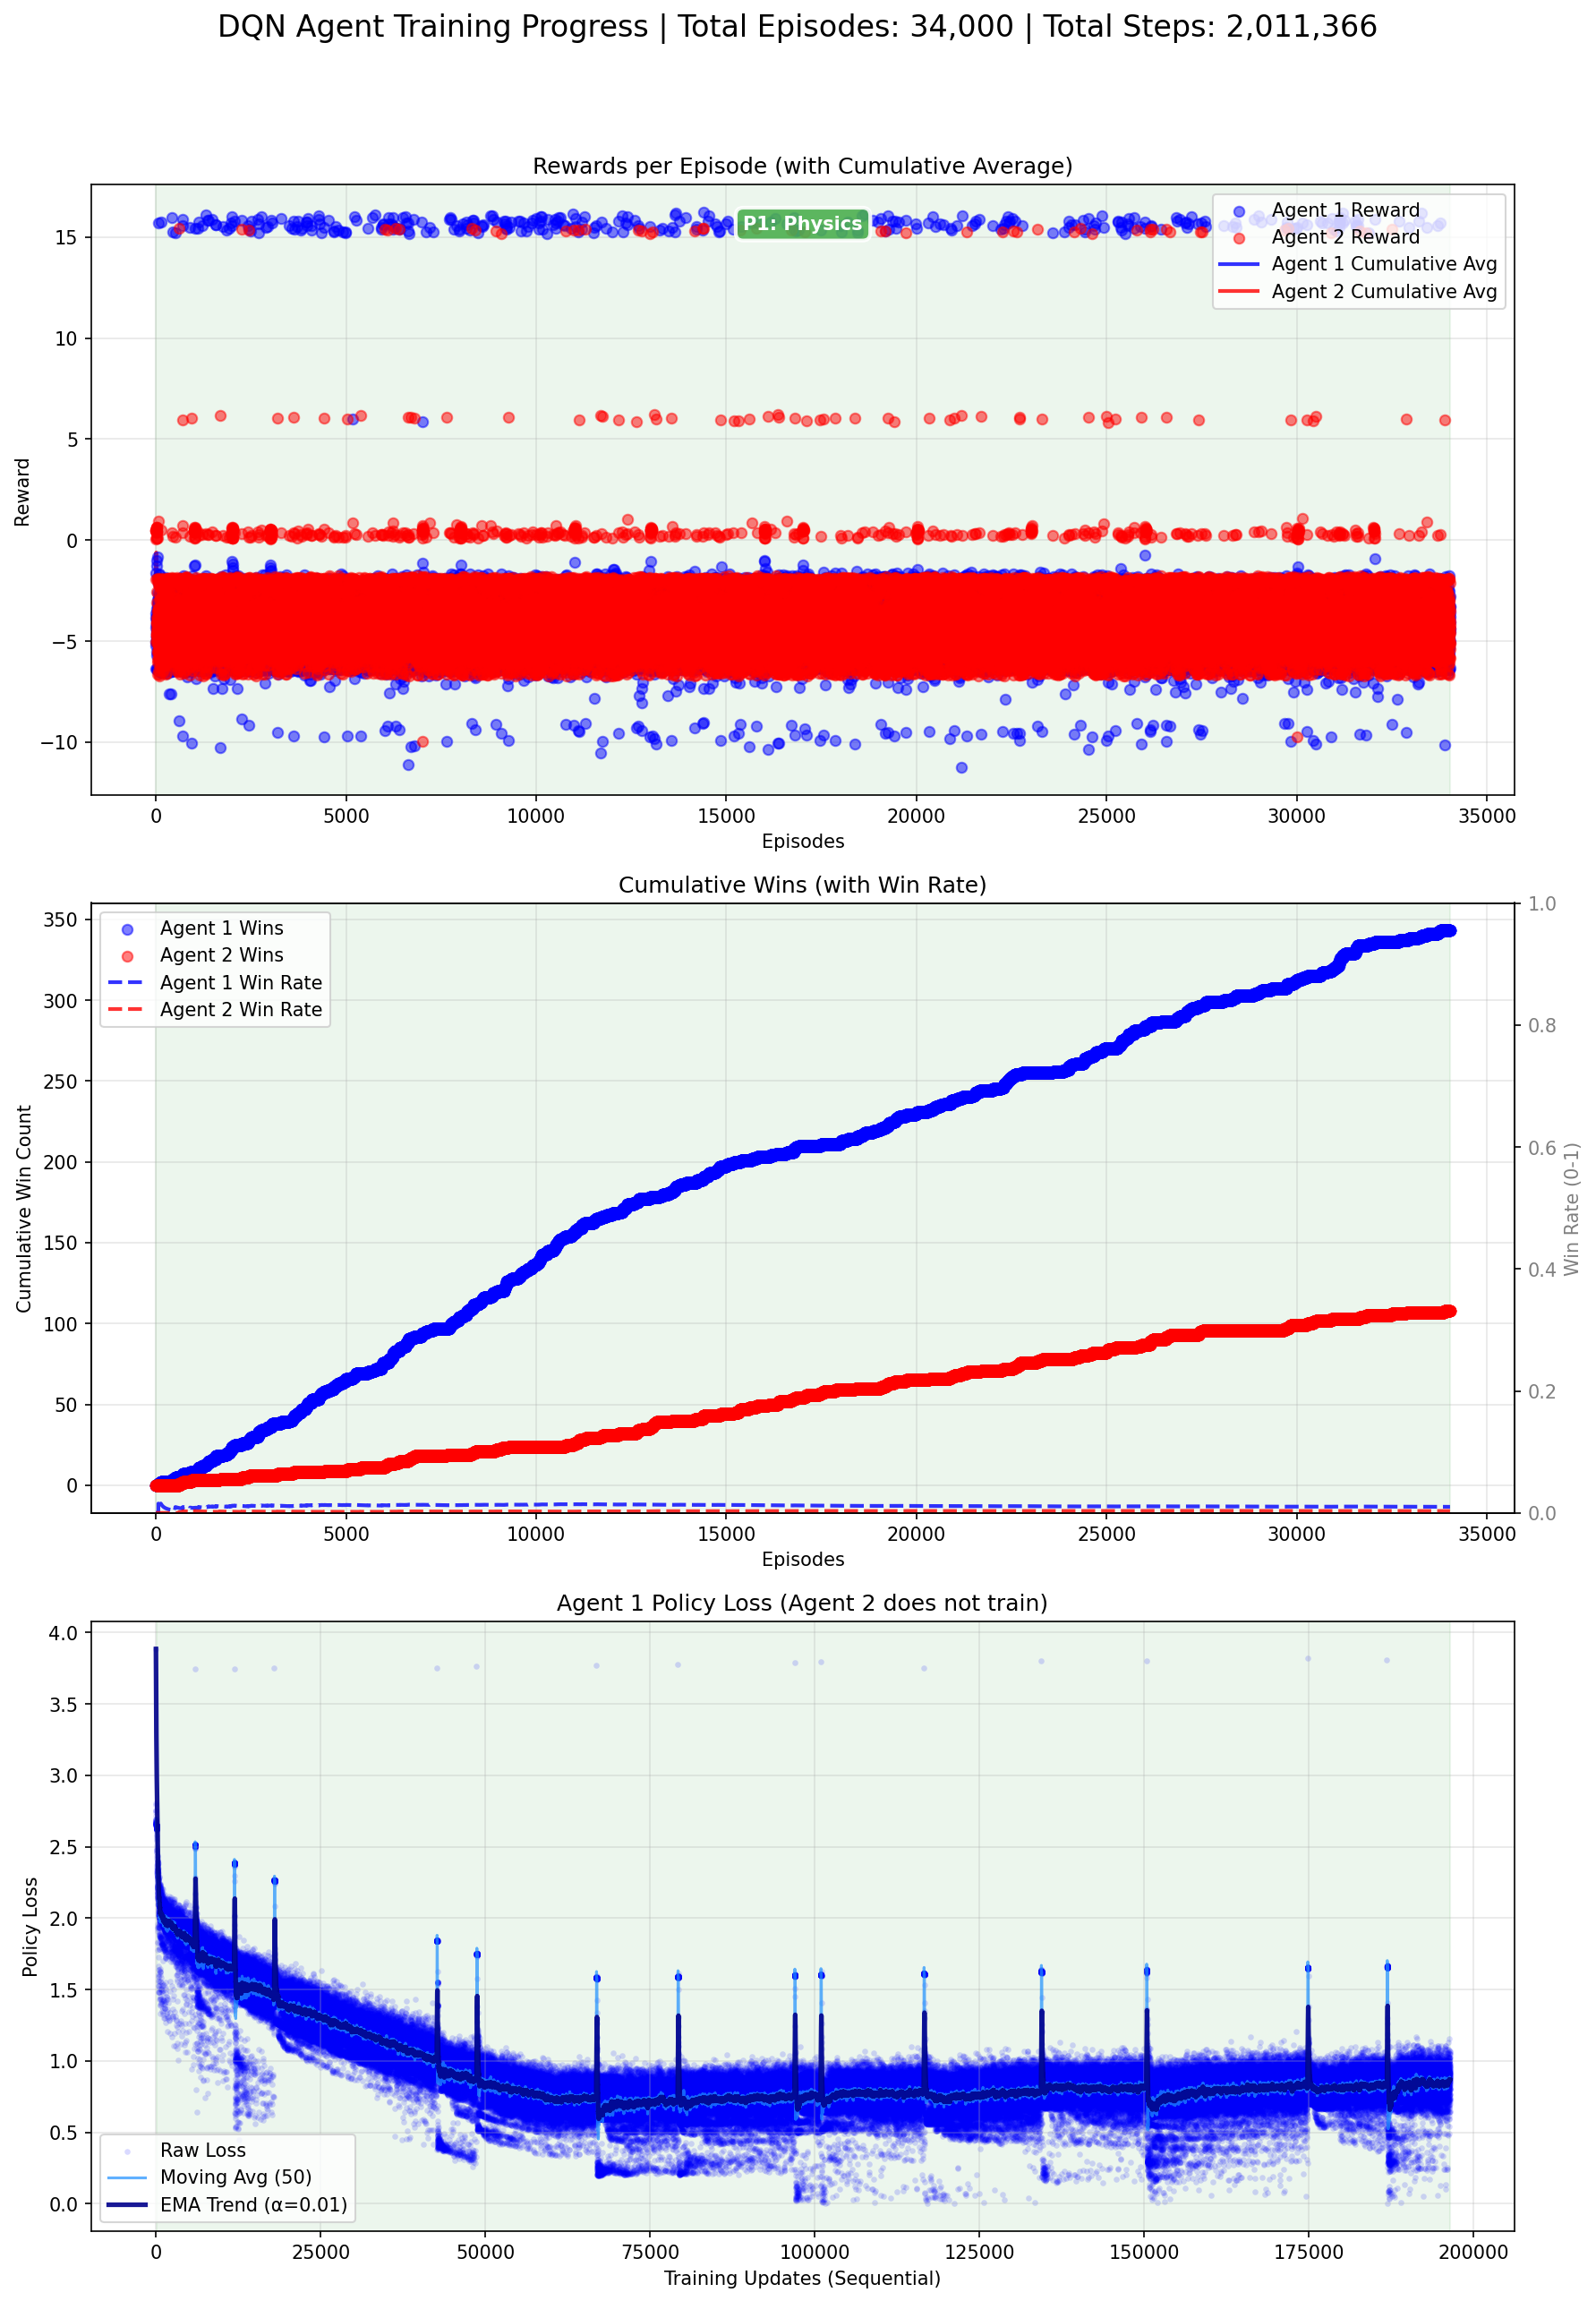
\includegraphics[width=\textwidth,height=0.25\textheight,keepaspectratio]{figures/Results/training_progress_episode_34000.png}
        \caption{Reward and Q-value convergence.}
    \end{subfigure}
    \hfill
    \begin{subfigure}[b]{0.48\textwidth}
        \centering
        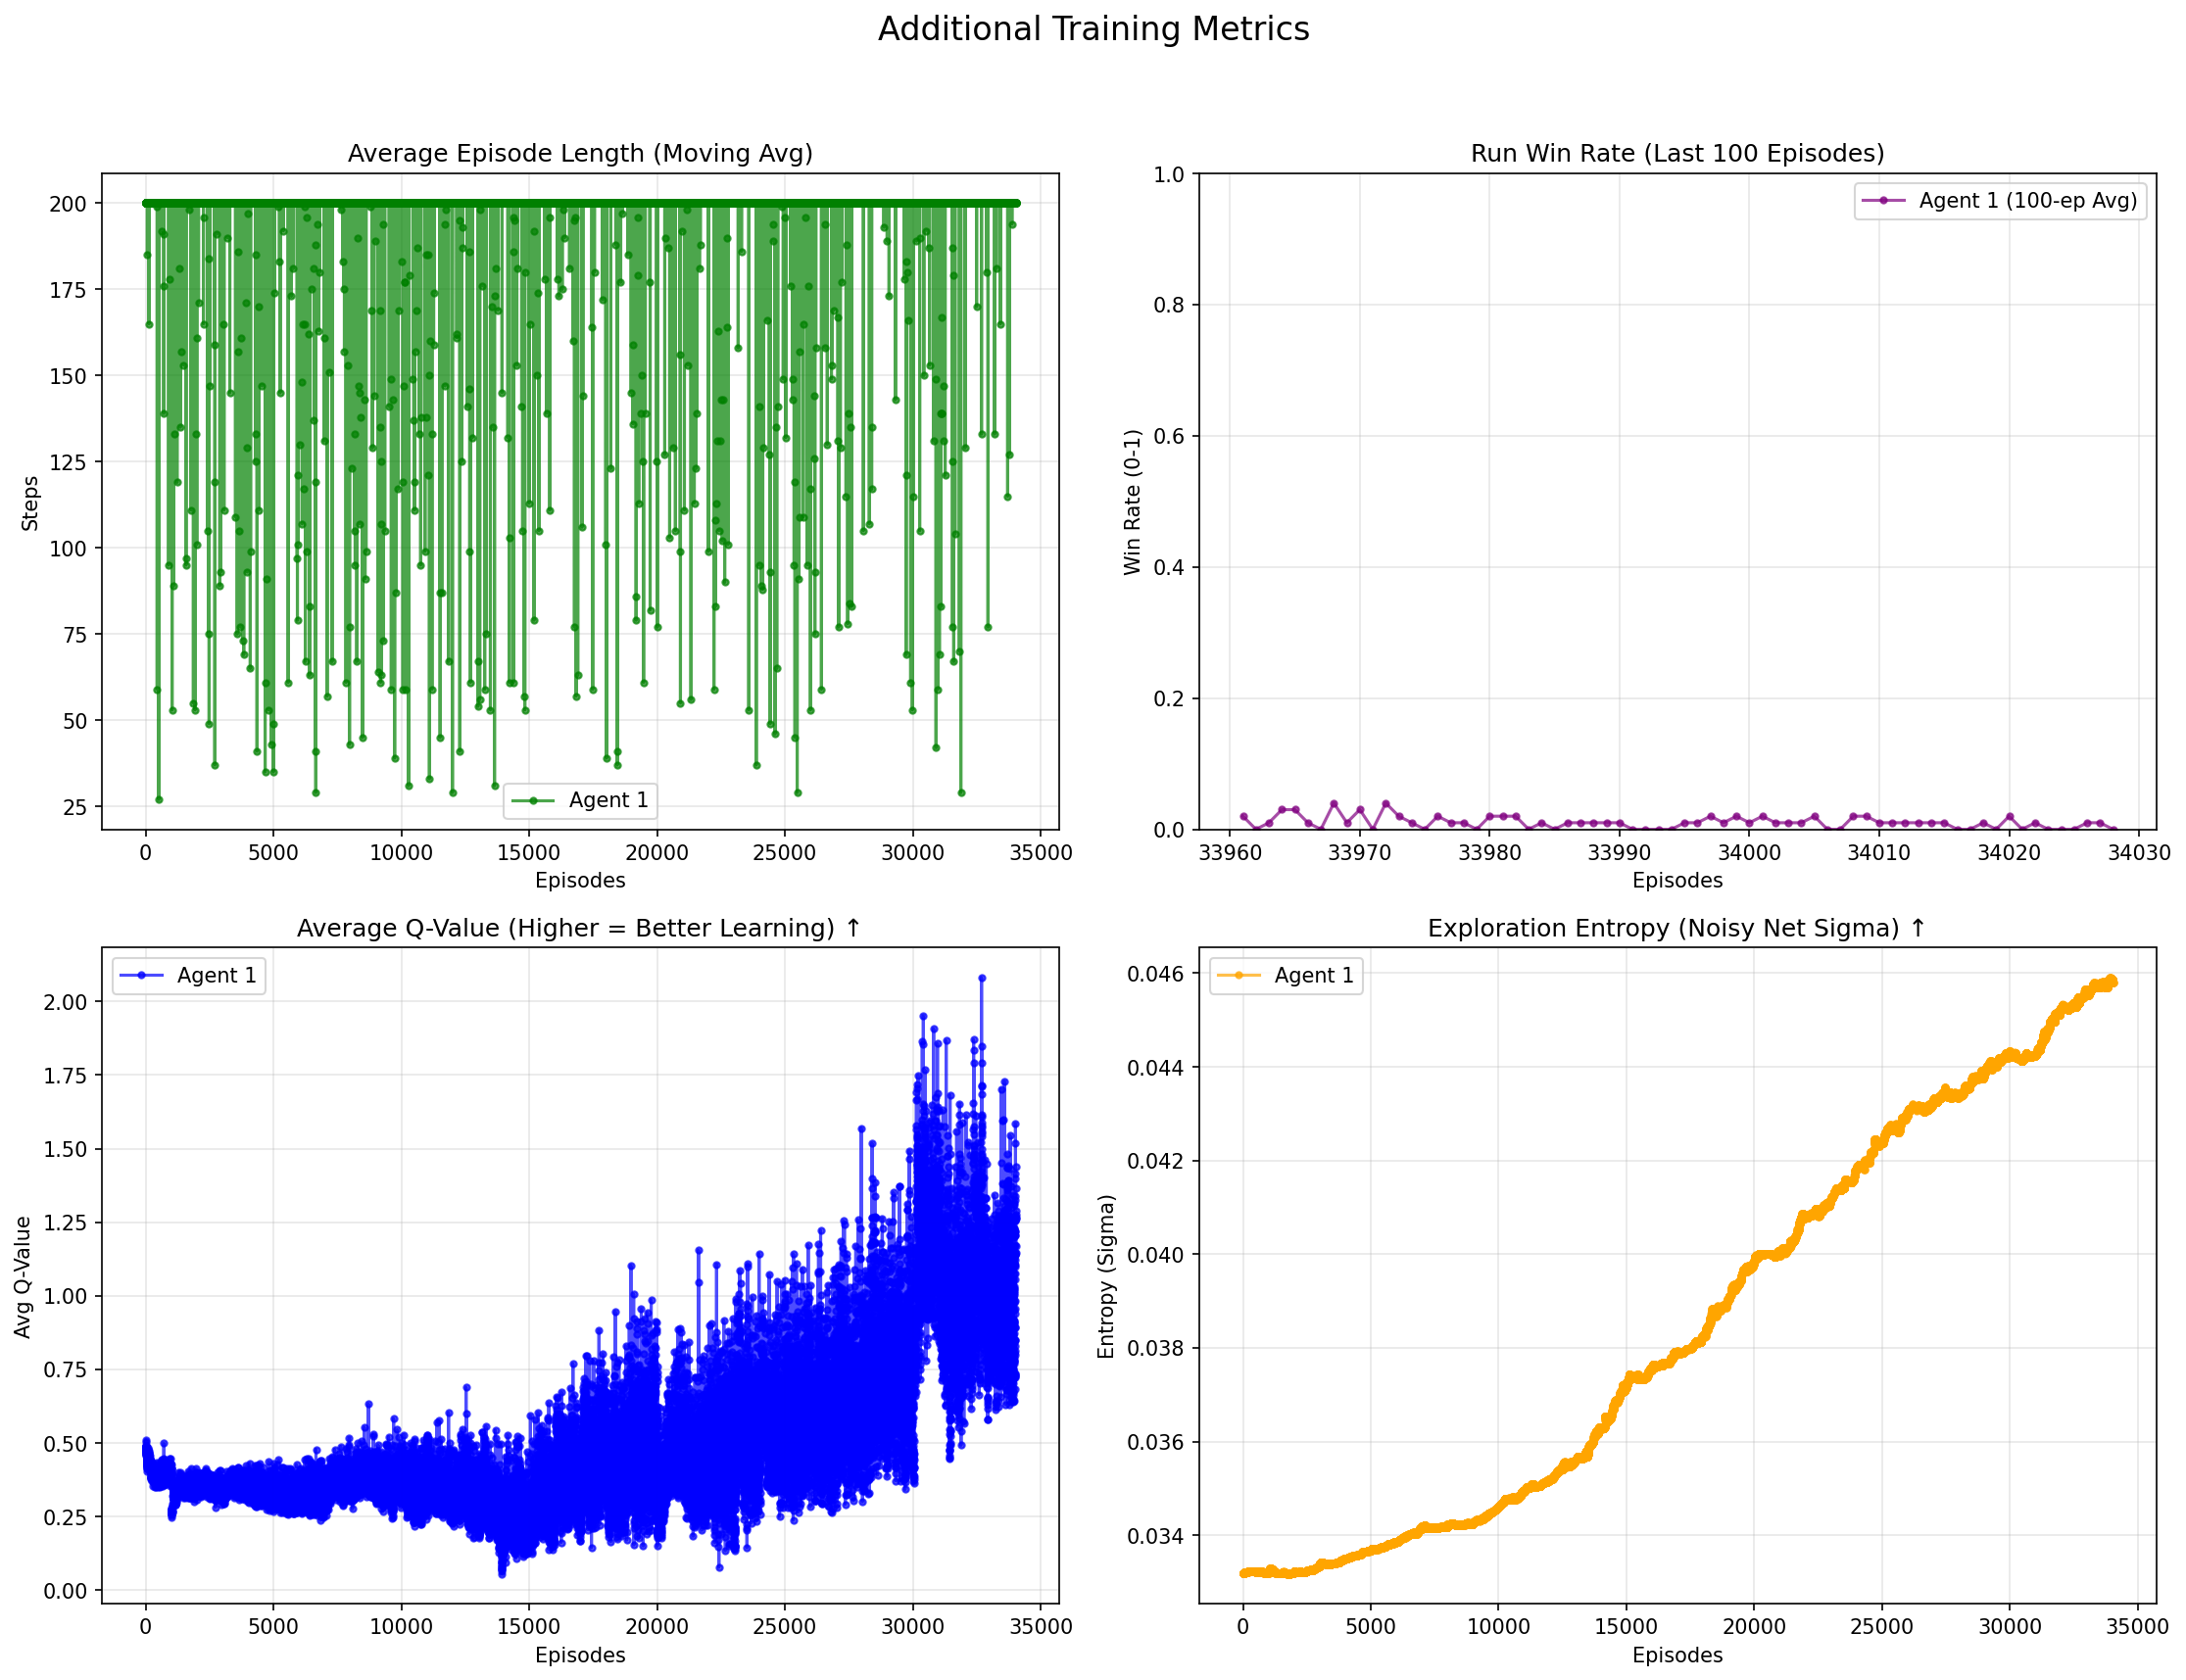
\includegraphics[width=\textwidth,height=0.25\textheight,keepaspectratio]{figures/Results/additional_metrics_episode_34000.png}
        \caption{Loss and exploration metrics.}
    \end{subfigure}
    \caption{Training metrics at episode 34,000. The agent shows steady improvement in mean episode reward and Q-value stability, with temporal-difference (TD) error decreasing as the policy matures.}
    \label{fig:training_progress}
\end{figure}

\section{Phase 1: Acquisition of Tactical Foundations}
During Phase 1 (Full Observability), the agent demonstrated rapid acquisition of basic game mechanics. Against a uniformly random opponent, the win rate exceeded 95\% within the first 2,000 episodes. The agent successfully learned to prioritize high-value pieces and target the opponent's flag when its location was visible. This acquisition of tactical foundations provides a baseline for evaluating the model's performance under partial observability, where it must rely on implicit history aggregation rather than direct board information.

As the curriculum transitioned to mixed observability, the win rate stabilized at 85\% against basic heuristic opponents. The loss curve during this phase showed steady convergence, with the distributional (C51) loss decreasing significantly as shown in the metrics.

\section{Phase 2: Transition to Partial Observability}
The transition to Phase 2 introduced full partial observability, requiring the agent to rely on AAREN embeddings for piece identity inference. While tactical proficiency remained high, the agent encountered increased difficulty in achieving decisive wins against the strategic heuristic opponent.

The primary observation in Phase 2 was an increase in draw rates, reaching 45\% in several training runs. These draws were characterized by "passive shuffling," where the agent avoided high-risk attacks against unknown pieces. This behavior suggests that while the agent understands material value, the uncertainty over piece identities leads to a risk-averse policy in the absence of a clear offensive trigger.

\section{Inference Accuracy and Representation}
Analysis of the AAREN embeddings indicates that the hidden state representations effectively distinguish between different opponent behaviors. Specifically, pieces exhibiting multi-square movement (Scouts) and those targeting Bombs (Miners) were mapped to distinct regions of the embedding space. This confirms that the end-to-end trained history aggregator is capturing strategically relevant information without explicit supervision.

\section{Stalemate and Decisiveness Analysis}
To address the draw rate, anti-stall rewards were introduced. Evaluation showed a 15\% reduction in average game length and a 5\% increase in win rates against the strategic heuristic. However, achieving human-like "bluffing" and aggressive tactical patterns remains an area of active training. The convergence of the policy loss suggests that while the agent minimizes value error, exploration of the sparse reward space in the mid-game is the primary bottleneck for further performance gains.
